% !TeX encoding = utf8
% !TeX spellcheck = en_GB

\section{Evaluation}

\subsection{Data Sets \label{sec:data-sets}}

As map data, we've used the data of the OpenStreetMap (OSM) project \parencite{OSMF2016}. Apart from the road network the data set contains for instance points of interest like shops (supermarkets, bakeries, etc.) or amenities (pharmacies,  toilets, etc.). Many of them are tagged with useful information e.g. on the accessibility (e.g. \verb|wheelchair=yes|) or their opening hours (e.g. \verb|opening_hours="MoSa 07:00-24:00; Su,PH off"|).

We used two different kind of weather data: the hourly air temperature and relative humidity values of a weather station alongside with to data sets of a thermal scanner flight.  

The hourly air temperature and relative humidity values are originating from the weather station of the German Weather Service (Deutscher Wetterdienste, DWD) in Rheinstetten near Karlsruhe \parencite{DWD2016}. Because only the hourly values have been available, the intermediate values haven been obtained using linear interpolation of the two adjacent values.

The other kind of data that we've used, have been remote sensing data of a thermal scanner flight provided by the Nachbarschaftsverband Karlsruhe (NVK). The data set consists of two scans, on recorded in the morning and on recorded in the evening of the 26 September 2008. The data are covering an area of  $\SI{25 805}{\meter} \times \SI{39 555}{\meter}$ (EW NS) an have a resolution of $5\,161 \times 7\,911$  pixels (pixel size \SI{}{\meter}). The measured surface temperature is in the range of \SIrange{-1.7}{18.3}{\celsius} (morning and evening). Before we used the data we rectified them using thin plate splines and cropped them to the same areas as the OSM data. The average surface temperature of the cropped data sets has been \SI{4.18}{\celsius} (morning) respectively \SI{11.24}{\celsius} evening.  


\subsection{Data Preparation}

\subsubsection{Routing}
Before extracting the road network, we cropped the OSM data set to the evaluated area. Afterwards, all ways tagged with \verb|highway|, \verb|railway=platform| or \verb|public_transport=platform| have been extracted.

 %In GraphHopper the edge weighting could be adapted for our needs. Additional the frame work provides implementation of many routing algorithms like Dijkstra's algorithm or the $A^*$ algorithm. Since we are only interested in pedestrian routing, we've used the \verb|FOOT| routing profile predefined in GraphHopper, which e.g. avoids certain highways like motorways.  

To compute the edge weights as described above in section \ref{sec:edge-weighting} we need to make some assumptions. That's because the weather data that we've used lacked either an appropriate spatial resolution (data of one weather station)  or the required temporal resolution (only two thermal scans). So, we've assumed that the actual spatial variation of the temperature conforms with the spatial variation of the thermal scans (deviation from the mean value). Because for the relative humidity no further data have been available, we assumed that there subject of any spatial variation. For the temporal variation, we've assumed that the temporal variation in the examined area correspond to the temporal variation measure at the weather station in Rheinstetten.  Additional we've used the thermal scan recorded in the morning for the time between 00:00 and 11:59 and the scan recorded in the evening for the time between 12:00 and 23:59.

So, we computed the air temperature at time $t\in T$ for the raster cell $c_{ij}$ as follows:
\begin{equation}
\label{eq:derived-temperature}
T_a(t, c_{ij}) = \begin{cases}
T_{a}^{station}(t) + \delta_{ij}^{morning} & \text{if $0 \leq t < 12$,}\\
T_{a}^{station}(t) + \delta_{ij}^{evening} & \text{if $12 \leq t < 24$,}
\end{cases}
\end{equation}
where $T_{a}^{station}(t)$ is the air temperature measured at the weather station at time $t$ and $\delta^{morning}_{ij}$ respectively  $\delta^{evening}_{ij}$ is the deviation of the raster cell $c_{ij}$ from the mean of all raster cells from the morning respectively evening scan.

To compute an approximation of Steadman's heat index we used the formula published by \textcite[77]{Stull2011}. Since the heat index is only defined for an air temperature between \SI{20}{\celsius} and \SI{50}{\celsius} we've used the air temperature as a fallback, if the air temperature was not within that range. Additionally, should be noted that if the air temperature respectively the heat index dropped in a raster cell below a comfort threshold $T_a^{comfort}$ or $T_{HI}^{comfort}$, then that comfort value has been used, because temperature below this threshold are not considered harmful. For both  $T_a^{comfort}$ or $T_{HI}^{comfort}$ we used \SI{20}{\celsius} as a threshold because temperatures above can cause a light heat stress \parencite{Staiger2011}.

For the actual implementation of the routing we used the GraphHopper framework for Java \parencite{GraphHopper2016,GraphHopper2016a}.

\subsubsection{Optimal Time}

To find an optimal point in time we used the procedure described in section \ref{sec:find-optimal-time}. As data we used the OSM data as well, because they contain the information necessary, i.e. points of interest with associated opening hours. 

For the nearby search,  we're using a list of selected OSM tags like \verb|shop=supermarket| or \verb|amenity=pharmacy| as a search criteria. We also only considering locations which have opening hours specified (via the \verb|opening_hours| tag). Additionally, only locations which are in a defined radius around the starting point are considered, at this we used the direct distance (“as the crow flies”). To reduce the computation effort a maximum number of results $k$ can be specified.

As optimization algorithm, we used implementation of Brent's method in the Apache Commons Mathematics Library \parencite{ASF2016} with 10 random start points to reduce the risk that only a local optimum is found.

If a shop is not opened over lunch, then for every time window (e.g. 9:00--13:00 and 14:00--18:30) an optimal time is determined and accordingly the solution with lowest heat exposure is used.

\subsection{Results}

\subsubsection{Routing}

\begin{figure}
	\centering
	\subfigure[map]{
		\label{fig:route-example:map}
		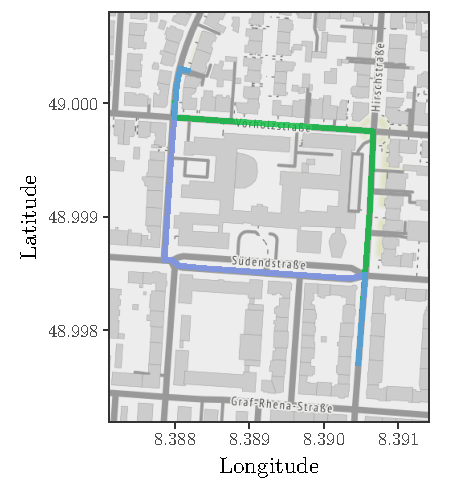
\includegraphics[scale=0.7]{figures/route_example_map}
	}    
	\subfigure[thermal scan (evening)]{
		\label{fig:route-example:raster}
		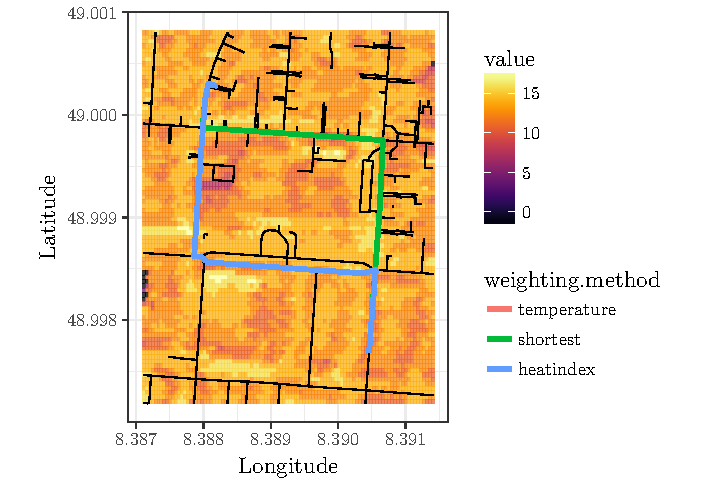
\includegraphics[scale=0.7]{figures/route_example_raster}
	}     
	\caption{Routing example: both the \emph{temperature} and the \emph{heatindex} weighting found the same route. (Map tiles by \textcite{Stamen2017}, under CC BY 3.0\protect\footnotemark. Map data by \textcite{OSMF2016}, under ODbL\protect\footnotemark)}
	\label{fig:route-example}
\end{figure}
\footnotetext{\url{http://creativecommons.org/licenses/by/3.0}}
\footnotetext{\url{http://www.openstreetmap.org/copyright}}

To evaluate the routing, we've selected 1000 random pairs of start and destinations points form the examined  area and 10 random dates from the period of 1 June to 31 August 2015. For each of the start destination pairs and each date we've performed the evaluation at 7:00, 11:00, 15:00, 19:00 and 23:00, so overall we had $50\,000$ samples. As edge weighting we've used the air temperature (equation \eqref{eq:edge-weight-temperature}, \emph{temperature})  and the heat index \eqref{eq:edge-weight-heatindex}, \emph{heatindex}). For comparison, we computed for each sample the shortest path. 

\begin{table}
	\centering
	\begin{tabular}{lp{8cm}lcc}
		\hline
		 & & temperature & heat index \\
		 \hline
		 \multicolumn{4}{l}{Reduction of heat exposure (\% of cases) }   \\
		& overall  & \SI{79.70}{\percent} & \SI{80.53}{\percent}  \\
		& more then \SI{5}{\percent} & \SI{42.72}{\percent} & \SI{45.11}{\percent} \\
		& more then \SI{10}{\percent} & \SI{13.81}{\percent} & \SI{16.07}{\percent} \\
		 \multicolumn{4}{l}{Reduction of heat exposure}  \\
		& average  & \SI{4.63}{\percent} & \SI{4.69}{\percent}  \\
		& maximum  & \SI{25.97}{\percent} & \SI{26.17 }{\percent}  \\
		\multicolumn{4}{l}{Increase of distance}  \\
		& \% of cases & \SI{93.81}{\percent} & \SI{94.11}{\percent}  \\
		& average & \SI{5.59}{\percent} & \SI{5.76}{\percent}  \\
		 \multicolumn{4}{l}{Reduction of relative heat exposure ($w_h / w_d$)}  \\
		 & average  & \SI{2.12}{\celsius} & \SI{2.32}{\celsius}  \\
		 \hline
	\end{tabular}
	\caption{Overview of the results of the routing approach. The values are relative to the shortest route. The relative heat exposure is a with the distance weighted average of the thermal comfort measure. That means, on average the heat exposure was about \SI{2}{\celsius} lower compared to the shortest route. \label{tab:results-routing}}
\end{table}

An overview of our results is given in table \ref{tab:results-routing}.

%The heat exposure compared to the shortest route could be reduced in \SI{79.70}{\percent} (\emph{temperature}) respectively  \SI{80.53}{\percent} of the cases. In \SI{42.72}{\percent} (\emph{temperature}; \emph{heatindex}: \SI{45.11}{\percent}) the heat exposure could be reduced by more than \SI{5}{\percent} and in \SI{13.81}{\percent} (\SI{16.07}{\percent}) of the cases by more the \SI{10}{\percent}. At best the heat exposure could be reduced by up to \SI{25.97}{\percent} (\emph{temperature}) respectively  \SI{26.17 }{\percent}. On average the relative heat exposure could be reduce by \SI{2.12}{\celsius} (\emph{temperature}) and \SI{ 2.32}{\celsius} (\emph{heatindex}). The relative heat exposure is the edge weight $w_{T_a}$ or $w_{HI}$ of the path normed on the path length $w_d$ and therefore a with the distance weighted average of the heat exposure. In \SI{93.81}{\percent} (\emph{heatindex}: \SI{94.11}{\percent}) of the cases a longer route was selected. On average the route with minimal heat exposure was \SI{5.59}{\percent} (\emph{temperature}) respectively  \SI{5.76}{\percent} (\emph{heatindex}) longer. 

An example can be seen in figure \ref{fig:route-example}. In this example the heat exposure could be reduced by \SI{17.64}{\percent} (\emph{temperature}) and \SI{18.76}{\percent} (\emph{heatindex}), while at the same time the distance only increased by  \SI{0.53}{\percent}.

\subsubsection{Optimal Time}

\begin{figure}
	\centering
	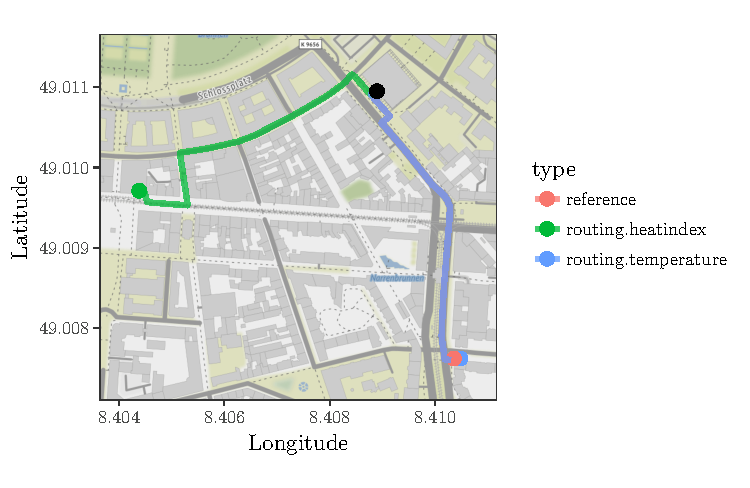
\includegraphics[scale=0.9]{figures/optimaltime_route_example}
	\caption{Example for nearby search: In the graphic the starting point (black dot) as well as the locations ranked first by the respective method. (Map tiles by \textcite{Stamen2017}, under CC BY 3.0. Map data by \textcite{OSMF2016}, under ODbL)}
	\label{fig:optimaltime-route-example}
\end{figure}

For the evaluation of optimal time finding procedure we selected 750 random start points. One of the following four search criteria has been assigned to each of the start points at random: supermarket, bakery, chemist or pharmacy. For each of the start points a random start time $t_{now}$ has been selected from the period of 8:00 to 20:00. The radius has been set to \SI{1000}{\meter} for all start points and the maximum number of results has been set to 5. Additionally, for all start points a time buffer $t_{buff}$ of 15 minutes has been assumed. 

As a reference solution, we've used the closest location found during the nearby search, computed the shortest path from the starting point to this location and evaluated the heat exposure at time $t_{now}$. The evaluation is performed only for the locations with rank 1, because those have the lowest heat exposure.

\begin{table}
	\centering
	\begin{tabular}{lp{8cm}lcc}
		\hline
		& & temperature & heat index \\
		\hline
		\multicolumn{4}{l}{Reduction of heat exposure}   \\
		& \% of cases  & \SI{68.43}{\percent} & \SI{71.08}{\percent}  \\
		\multicolumn{4}{l}{Reduction of heat exposure}  \\
		& average  & \SI{8.09}{\percent} & \SI{7.73}{\percent}  \\
		& maximum  & \SI{62.29}{\percent} & \SI{62.88}{\percent}  \\
		\multicolumn{4}{l}{Increase of distance}  \\
		& average  & \SI{4.60}{\percent}  & \SI{4.72}{\percent}  \\
		\hline
	\end{tabular}
	\caption{Overview of the results of the combined approach each compared with the reference solution.  \label{tab:results-optima-time}}
\end{table}


The heat exposure could be reduced in \SI{68.43}{\percent} (\emph{temperature}) respectively \SI{71.08}{\percent} by up to \SI{62.29}{\percent} (\SI{62.88}{\percent}). On average the heat exposure could be reduced by \SI{8.09}{\percent} (\emph{temperature}) and \SI{7.73}{\percent}. The average increase of the distance was \SI{4.60}{\percent} and \SI{4.72}{\percent}.

An example can be seen in figure \ref{fig:optimaltime-route-example}. 
Here the \emph{temperature} weighting selected the same pharmacy and optimal point in time (9:27) as the reference solution. Contrary the \emph{heatindex} routing selected a different pharmacy which is \SI{476.6}{\meter} instead of  \SI{434.5}{\meter} a way from the starting point. Additional the method found a different optimal time (19:39) and those the heat exposure could be reduced by \SI{18.49}{\percent}.  
 
